\chapter{Échecs et projets avortés}
\label{section:avortes}

\section{Interconnexion de systèmes}

\paragraph{}
Au début de mon stage, il était question de construire une architecture permettant d'interconnecter divers outils souvent intégrés chez les clients de la \abusys.
La communication mise en place aurait permis aux différents systèmes d'échanger des données entre eux de façon à créer un \og meta-système \fg{} composé de plusieurs outils.

\paragraph{}
Intuitivement, je me suis documenté sur le concept d'Enterprise Service Bus (ESB) que l'on m'avait évoqué dans quelques cours lors de ma formation à l'UTC.
Ces ESB permettent justement la communication entre applications qui à la base ne sont pas pensées pour fonctionner ensemble.
Dans le principe, chaque application est enrobée dans un conteneur de service développé spécifiquement pour l'ESB choisi.
Ensuite, les conteneurs de services communiquent entre eux via des protocoles standards comme XML, JMS ou les services web.

J'ai commencé par prendre en main l'ESB \apetals{} mais rapidement, nous avons compris que l'ESB était une technologie difficile à maîtriser sans formation.
La maintenance ultérieure de l'architecture aurait été trop lourde pour la \abusys.

\paragraph{}
L'idée alternative était de développer de A à Z la solution d'interconnexion en langage Python.
J'ai commencé à réaliser ce nouveau système pendant deux semaines.
Finalement, le projet a été abandonné car de nouvelles priorités sont apparues dans la \abusys.
On m'a demandé de travailler sur d'autres projets plus urgents et de moins grande envergure pour le compte de clients ou pour les besoins internes de l'entreprise.



\section{Livre blanc sur l'offre \og plateformes d'intégration continue \fg}

\paragraph{}
Une idée pour concrétiser mon sujet de stage était de rédiger une ébauche de livre blanc\footnote{\asmile{} est une entreprise très populaire grâce aux différents livres blancs qu'elle a déjà publiés. Ces livres portent sur un certain nombre de domaines liés à l'informatique, comme les bonnes pratiques du web ou les pare-feux open source. Les lecteurs apprécient entre autres la vue d'ensemble des solutions du marché qui y est donnée.}.
Une fois finalisé, celui-ci aurait éventuellement été publié sur le site web de \asmile.
Cela aurait permis de promouvoir l'offre \og plateformes d'intégration continue \fg{} proposée par \asmile{} afin de démontrer un savoir-faire et gagner de nouveaux clients.

\paragraph{}
Dans ce cas aussi, les priorités ont rattrapé le projet.
Il était urgent que j'intervienne en tant que soutien au développement d'un projet client en retard pour \abt{} évoqué précédemment.
Ce projet a donc été lui aussi abandonné.



\section{Solution de vidéoconférence}

\paragraph{}
Mon manager \apakou{} m'a confié la mission de tenter de mettre en place une telle solution via le produit open source OpenMCU.
Destinée à des besoins internes de \asmile, cette plateforme aurait servi à remplacer la solution actuellement en place -- coûteuse et ne répondant pas aux qualités de services attendues -- afin d'organiser des réunion inter-agences à distance.

\paragraph{}
OpenMCU prend la forme d'un démon\footnote{Un \etranger{daemon} ou démon désigne un type de programme informatique, un processus qui s'exécute en arrière-plan plutôt que sous le contrôle direct d'un utilisateur. Les démons sont souvent démarrés lors du chargement du système d'exploitation, et servent en général à répondre à des requêtes du réseau, à l'activité du matériel ou à d'autres programmes en exécutant certaines tâches.~\cite{demon}} acceptant les connexions de clients respectant la norme H.323\footnote{H.323 regroupe un ensemble de protocoles de communication de la voix, de l'image et de données sur IP. C'est un protocole développé par l'UIT-T qui le définit comme : \og Systèmes de communication multimédia en mode paquet \fg.~\cite{h323}}.
Ainsi, les utilisateurs qui se connectent au service se rencontrent dans une salle de discussion.
Du point de vue audio, tous les participants peuvent s'entendre et communiquer entre eux.
Du côté de la vidéo, chaque participant transmet son propre flux vidéo. Celui-ci est retransmis à tout le monde sous la forme d'une seule vidéo scindée en plusieurs parties, chacune représentant le flux vidéo de chaque participant (\cffigure{stage:openmcu}).

\begin{figure}
	\centering
	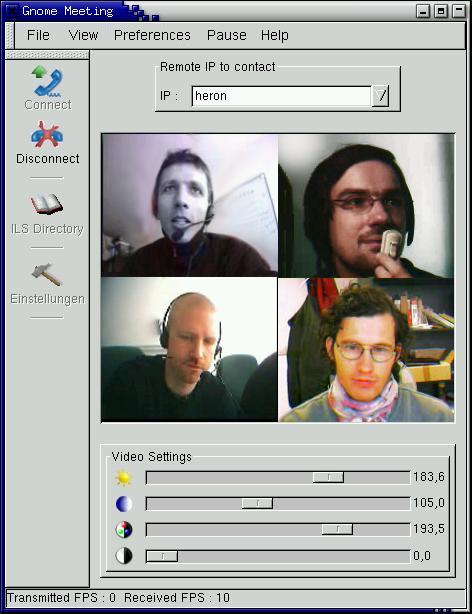
\includegraphics[height=5.5cm]{stage/openmcu}
	\caption{Exemple d'utilisation de la solution de vidéoconférence OpenMCU}
	\label{figure:stage:openmcu}
\end{figure}

\paragraph{}
Finalement, je n'ai pas réussi à mettre en place la solution, faute de documentation et de support sur le produit.
La qualité de son était assez faible et la vidéo ne fonctionnait pas.
Finalement, il a été possible de répondre au besoin grâce la solution de web-conférence BigBlueButton (\cffigure{stage:bbb}), plus récente et mieux supportée, que j'ai pu mettre en place avec succès.

\begin{figure}[htb]
	\centering
	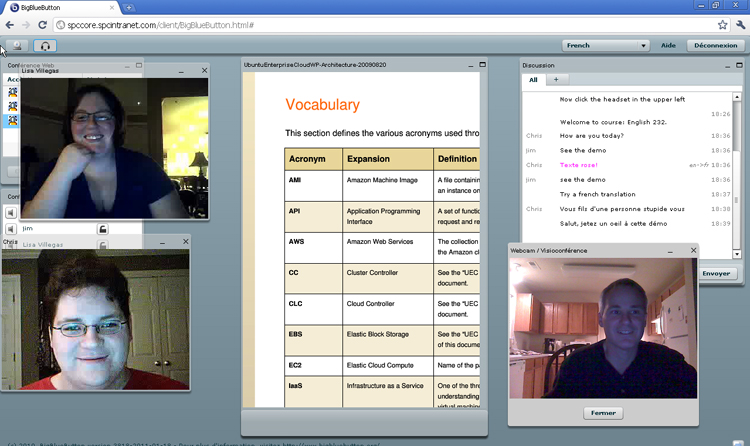
\includegraphics[width=13cm]{stage/bbb}
	\caption{Exemple d'utilisation de la solution de web-conférence BigBlueButton}
	\label{figure:stage:bbb}
\end{figure}

